\documentclass{standalone}

%%% Schrift auswählen
\usepackage{XCharter}
\usepackage{FiraSans}
\usepackage{fontspec}
\setmonofont{DejaVu Sans Mono}[Scale=0.9]
%\setmonofont{inconsolata}
%\setmonofont{JetBrains Mono}
\setmainfont{XCharter}
\newfontfamily{\lato}{Lato}

\usepackage{tikz}
\usetikzlibrary{positioning, arrows.meta}
\usetikzlibrary{fit}

\begin{document}

\begin{tikzpicture}[font=\LARGE]
    %%% Pointer-Stil
    % Definiere Stil für einen Pointer-Punkt
    \tikzstyle{pointer} = [circle, fill, inner sep=3pt]
    % Definiere Stil für einen Pointer-Pfeil
    \tikzstyle{arrow} = [->, thick, >=Latex, >={Latex[length=5mm, width=3mm]}]

    % Player[0] bestehend aus firstName, lastName und age
    \node[draw=none, inner sep=0pt, outer sep=0pt] (player0) {
        \begin{tikzpicture}
        %%% First element
            % Define a node with transparent bottom side
            \node[draw=none, minimum width=2cm, minimum height=1.5cm, inner sep=0pt, outer sep=0pt] (1rectLeft) {};

            % Draw the visible sides of the rectangle
            \draw (1rectLeft.north west) -- (1rectLeft.north east); % Top side
            \draw (1rectLeft.north west) -- (1rectLeft.south west); % Left side
            %\draw (1rectLeft.north east) -- (1rectLeft.south east); % Right side empty
            \draw (1rectLeft.south west) -- (1rectLeft.south east); % Bottom side

            % Define a node with transparent left and right sides, positioned directly right of 1rectLeft
            \node[draw=none, minimum width=2cm, minimum height=1.5cm, inner sep=0pt, outer sep=0pt, right=0 of 1rectLeft] (1rectMiddle) {\texttt{firstName}};

            % Draw the dashed top and bottom sides
            \draw[dashed] (1rectMiddle.north west) -- (1rectMiddle.north east); % Top side
            \draw[dashed] (1rectMiddle.south west) -- (1rectMiddle.south east); % Bottom side

            % Transparent left and right sides (using white color to match the background)
            \draw[white] (1rectMiddle.south west) -- (1rectMiddle.north west); % left side
            \draw[white] (1rectMiddle.south east) -- (1rectMiddle.north east); % right side

            % Define a node with transparent left side
            \node[draw=none, minimum width=2cm, minimum height=1.5cm, inner sep=0pt, outer sep=0pt, right=0 of 1rectMiddle] (1rectRight) {};

            % Draw the visible sides of the rectangle
            \draw (1rectRight.north west) -- (1rectRight.north east); % Top side
            %\draw (1rectRight.north west) -- (1rectRight.south west); % Left side
            \draw (1rectRight.north east) -- (1rectRight.south east); % Right side
            \draw (1rectRight.south west) -- (1rectRight.south east); % Bottom side

        %%% Second element
            % Define a node with transparent right side
            \node[draw=none, minimum width=2cm, minimum height=1.5cm, inner sep=0pt, outer sep=0pt, right=0 of 1rectRight] (2rectLeft) {};

            % Draw the visible sides of the rectangle
            \draw (2rectLeft.north west) -- (2rectLeft.north east); % Top side
            \draw (2rectLeft.north west) -- (2rectLeft.south west); % Left side
            %\draw (2rectLeft.north east) -- (2rectLeft.south east); % Right side
            \draw (2rectLeft.south west) -- (2rectLeft.south east); % Top side

            % Define a node with transparent left and right sides, positioned directly left to 2rectLeft
            \node[draw=none, minimum width=2cm, minimum height=1.5cm, inner sep=0pt, outer sep=0pt, right=0 of 2rectLeft] (2rectMiddle) {\texttt{lastName}};

            % Draw the dashed top and bottom sides
            \draw[dashed] (2rectMiddle.north west) -- (2rectMiddle.north east); % Top side
            \draw[dashed] (2rectMiddle.south west) -- (2rectMiddle.south east); % Bottom side

            % Transparent left and right sides (using white color to match the background)
            \draw[white] (2rectMiddle.south west) -- (2rectMiddle.north west); % Left side
            \draw[white] (2rectMiddle.south east) -- (2rectMiddle.north east); % Right side

            % Define a node with transparent left side
            \node[draw=none, minimum width=2cm, minimum height=1.5cm, inner sep=0pt, outer sep=0pt, right=0 of 2rectMiddle] (2rectRight) {};

            % Draw the visible sides of the rectangle
            \draw (2rectRight.north west) -- (2rectRight.north east); % Top side
            %\draw (2rectRight.north west) -- (2rectRight.south west); % Left side
            \draw (2rectRight.north east) -- (2rectRight.south east); % Right side
            \draw (2rectRight.south west) -- (2rectRight.south east); % Bottom side

        %%% Third element
            % Define a node with fully visible sides of the rectangle
            \node[draw, minimum width=2cm, minimum height=1.5cm, inner sep=0pt, outer sep=0pt, right=0 of 2rectRight] (3rect) {\texttt{age}};
        \end{tikzpicture}
    };

    % Player[1] bestehend aus firstName, lastName und age
    \node[draw=none, inner sep=0pt, outer sep=0pt, below=0.2cm of player0] (player1) {
        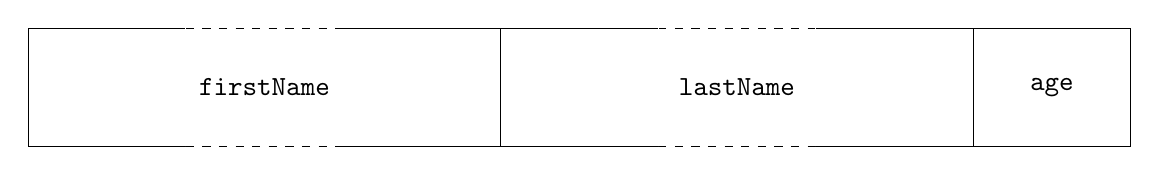
\begin{tikzpicture}
        %%% First element
            % Define a node with transparent bottom side
            \node[draw=none, minimum width=2cm, minimum height=1.5cm, inner sep=0pt, outer sep=0pt] (1rectLeft) {};

            % Draw the visible sides of the rectangle
            \draw (1rectLeft.north west) -- (1rectLeft.north east); % Top side
            \draw (1rectLeft.north west) -- (1rectLeft.south west); % Left side
            %\draw (1rectLeft.north east) -- (1rectLeft.south east); % Right side empty
            \draw (1rectLeft.south west) -- (1rectLeft.south east); % Bottom side

            % Define a node with transparent left and right sides, positioned directly right of 1rectLeft
            \node[draw=none, minimum width=2cm, minimum height=1.5cm, inner sep=0pt, outer sep=0pt, right=0 of 1rectLeft] (1rectMiddle) {\texttt{firstName}};

            % Draw the dashed top and bottom sides
            \draw[dashed] (1rectMiddle.north west) -- (1rectMiddle.north east); % Top side
            \draw[dashed] (1rectMiddle.south west) -- (1rectMiddle.south east); % Bottom side

            % Transparent left and right sides (using white color to match the background)
            \draw[white] (1rectMiddle.south west) -- (1rectMiddle.north west); % left side
            \draw[white] (1rectMiddle.south east) -- (1rectMiddle.north east); % right side

            % Define a node with transparent left side
            \node[draw=none, minimum width=2cm, minimum height=1.5cm, inner sep=0pt, outer sep=0pt, right=0 of 1rectMiddle] (1rectRight) {};

            % Draw the visible sides of the rectangle
            \draw (1rectRight.north west) -- (1rectRight.north east); % Top side
            %\draw (1rectRight.north west) -- (1rectRight.south west); % Left side
            \draw (1rectRight.north east) -- (1rectRight.south east); % Right side
            \draw (1rectRight.south west) -- (1rectRight.south east); % Bottom side

        %%% Second element
            % Define a node with transparent right side
            \node[draw=none, minimum width=2cm, minimum height=1.5cm, inner sep=0pt, outer sep=0pt, right=0 of 1rectRight] (2rectLeft) {};

            % Draw the visible sides of the rectangle
            \draw (2rectLeft.north west) -- (2rectLeft.north east); % Top side
            \draw (2rectLeft.north west) -- (2rectLeft.south west); % Left side
            %\draw (2rectLeft.north east) -- (2rectLeft.south east); % Right side
            \draw (2rectLeft.south west) -- (2rectLeft.south east); % Top side

            % Define a node with transparent left and right sides, positioned directly left to 2rectLeft
            \node[draw=none, minimum width=2cm, minimum height=1.5cm, inner sep=0pt, outer sep=0pt, right=0 of 2rectLeft] (2rectMiddle) {\texttt{lastName}};

            % Draw the dashed top and bottom sides
            \draw[dashed] (2rectMiddle.north west) -- (2rectMiddle.north east); % Top side
            \draw[dashed] (2rectMiddle.south west) -- (2rectMiddle.south east); % Bottom side

            % Transparent left and right sides (using white color to match the background)
            \draw[white] (2rectMiddle.south west) -- (2rectMiddle.north west); % Left side
            \draw[white] (2rectMiddle.south east) -- (2rectMiddle.north east); % Right side

            % Define a node with transparent left side
            \node[draw=none, minimum width=2cm, minimum height=1.5cm, inner sep=0pt, outer sep=0pt, right=0 of 2rectMiddle] (2rectRight) {};

            % Draw the visible sides of the rectangle
            \draw (2rectRight.north west) -- (2rectRight.north east); % Top side
            %\draw (2rectRight.north west) -- (2rectRight.south west); % Left side
            \draw (2rectRight.north east) -- (2rectRight.south east); % Right side
            \draw (2rectRight.south west) -- (2rectRight.south east); % Bottom side

        %%% Third element
            % Define a node with fully visible sides of the rectangle
            \node[draw, minimum width=2cm, minimum height=1.5cm, inner sep=0pt, outer sep=0pt, right=0 of 2rectRight] (3rect) {\texttt{age}};
        \end{tikzpicture}
    };

    % Player[2] bestehend aus firstName, lastName und age
    \node[draw=none, inner sep=0pt, outer sep=0pt, below=0.2cm of player1] (player2) {
        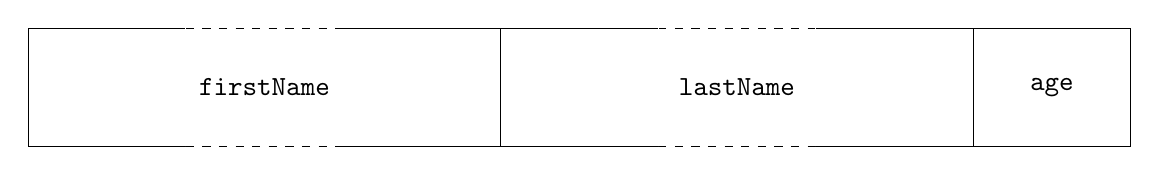
\begin{tikzpicture}
        %%% First element
            % Define a node with transparent bottom side
            \node[draw=none, minimum width=2cm, minimum height=1.5cm, inner sep=0pt, outer sep=0pt] (1rectLeft) {};

            % Draw the visible sides of the rectangle
            \draw (1rectLeft.north west) -- (1rectLeft.north east); % Top side
            \draw (1rectLeft.north west) -- (1rectLeft.south west); % Left side
            %\draw (1rectLeft.north east) -- (1rectLeft.south east); % Right side empty
            \draw (1rectLeft.south west) -- (1rectLeft.south east); % Bottom side

            % Define a node with transparent left and right sides, positioned directly right of 1rectLeft
            \node[draw=none, minimum width=2cm, minimum height=1.5cm, inner sep=0pt, outer sep=0pt, right=0 of 1rectLeft] (1rectMiddle) {\texttt{firstName}};

            % Draw the dashed top and bottom sides
            \draw[dashed] (1rectMiddle.north west) -- (1rectMiddle.north east); % Top side
            \draw[dashed] (1rectMiddle.south west) -- (1rectMiddle.south east); % Bottom side

            % Transparent left and right sides (using white color to match the background)
            \draw[white] (1rectMiddle.south west) -- (1rectMiddle.north west); % left side
            \draw[white] (1rectMiddle.south east) -- (1rectMiddle.north east); % right side

            % Define a node with transparent left side
            \node[draw=none, minimum width=2cm, minimum height=1.5cm, inner sep=0pt, outer sep=0pt, right=0 of 1rectMiddle] (1rectRight) {};

            % Draw the visible sides of the rectangle
            \draw (1rectRight.north west) -- (1rectRight.north east); % Top side
            %\draw (1rectRight.north west) -- (1rectRight.south west); % Left side
            \draw (1rectRight.north east) -- (1rectRight.south east); % Right side
            \draw (1rectRight.south west) -- (1rectRight.south east); % Bottom side

        %%% Second element
            % Define a node with transparent right side
            \node[draw=none, minimum width=2cm, minimum height=1.5cm, inner sep=0pt, outer sep=0pt, right=0 of 1rectRight] (2rectLeft) {};

            % Draw the visible sides of the rectangle
            \draw (2rectLeft.north west) -- (2rectLeft.north east); % Top side
            \draw (2rectLeft.north west) -- (2rectLeft.south west); % Left side
            %\draw (2rectLeft.north east) -- (2rectLeft.south east); % Right side
            \draw (2rectLeft.south west) -- (2rectLeft.south east); % Top side

            % Define a node with transparent left and right sides, positioned directly left to 2rectLeft
            \node[draw=none, minimum width=2cm, minimum height=1.5cm, inner sep=0pt, outer sep=0pt, right=0 of 2rectLeft] (2rectMiddle) {\texttt{lastName}};

            % Draw the dashed top and bottom sides
            \draw[dashed] (2rectMiddle.north west) -- (2rectMiddle.north east); % Top side
            \draw[dashed] (2rectMiddle.south west) -- (2rectMiddle.south east); % Bottom side

            % Transparent left and right sides (using white color to match the background)
            \draw[white] (2rectMiddle.south west) -- (2rectMiddle.north west); % Left side
            \draw[white] (2rectMiddle.south east) -- (2rectMiddle.north east); % Right side

            % Define a node with transparent left side
            \node[draw=none, minimum width=2cm, minimum height=1.5cm, inner sep=0pt, outer sep=0pt, right=0 of 2rectMiddle] (2rectRight) {};

            % Draw the visible sides of the rectangle
            \draw (2rectRight.north west) -- (2rectRight.north east); % Top side
            %\draw (2rectRight.north west) -- (2rectRight.south west); % Left side
            \draw (2rectRight.north east) -- (2rectRight.south east); % Right side
            \draw (2rectRight.south west) -- (2rectRight.south east); % Bottom side

        %%% Third element
            % Define a node with fully visible sides of the rectangle
            \node[draw, minimum width=2cm, minimum height=1.5cm, inner sep=0pt, outer sep=0pt, right=0 of 2rectRight] (3rect) {\texttt{age}};
        \end{tikzpicture}
    };

    % Speicherzellen für team-Array mit den Elementen team[0] bis team[2]
    \node[draw, minimum size=1.5cm, inner sep=0pt, outer sep=0pt, left=1 of player0] (team0) {};
    \node[left=0.5cm of team0] (text_team0) {\texttt{team[0]}};

    \node[draw, minimum size=1.5cm, inner sep=0pt, outer sep=0pt, left=1 of player1] (team1) {};
    \node[left=0.5cm of team1] (text_team1) {\texttt{team[1]}};

    \node[draw, minimum size=1.5cm, inner sep=0pt, outer sep=0pt, left=1 of player2] (team2) {};
    \node[left=0.5cm of team2] (text_team2) {\texttt{team[2]}};

    % Pointer von team0 auf player0
    \node[pointer] (pointer0) at (team0) {};
    \draw[arrow] (pointer0) -- (player0.west);

    % Pointer von team1 auf player1
    \node[pointer] (pointer1) at (team1) {};
    \draw[arrow] (pointer1) -- (player1.west);

    % Pointer von team2 auf player2
    \node[pointer] (pointer2) at (team2) {};
    \draw[arrow] (pointer2) -- (player2.west);

    % Speicherzelle für team-Pointer-Pointer
    \node[draw, minimum size=1.5cm, inner sep=0pt, outer sep=0pt, above=3 of team0] (team) {};
    \node[left=0.5cm of team] (text_team) {\texttt{team}};

    % Pointer auf das team-Array
    \node[pointer] (pointer_team) at (team) {};
    \draw[arrow] (pointer_team.south) -- (team0.north);

    % Rectangle around the nodes with a small inner distance
    \node[draw, dotted, rectangle, inner sep=3pt, fit=(team0)(team1)(team2), line width=0.3mm] {};

\end{tikzpicture}

\end{document}
